\documentclass[
 paper=A4,pagesize=automedia,fontsize=12pt,
 BCOR=15mm,DIV=22,
 twoside,headinclude,footinclude=false,
 fleqn,                     % fleqn = linksbündige Ausrichtung von Formeln
 bibtotocnumbered,          % Literaturverz. im Inhaltsverz. eintragen
 liststotoc,                % Abbildungsverz. im Inhaltsverz. eintragen
 listsleft,                 % Abbildungsverz. an der längsten Nummer ausrichten
 %pointlessnumbers,          % kein Punkt nach Überschriftsnummerierung
 cleardoublepage=empty      % Vakatseiten ohne Paginierung
]{scrbook}
\setlength\parindent{0em}

% Kodierung, Schrift und Sprache auswählen
\usepackage[utf8]{inputenc}
\usepackage[T1]{fontenc}
\usepackage{babel}
% damit man Text aus dem PDF korrekt rauskopieren kann
\usepackage{cmap}
% Layout: Kopf-/Fußzeilen, anderthalbfacher Zeilenabstand
\usepackage{scrpage2} \pagestyle{scrheadings}
                      \clearscrheadfoot
                      \ihead{\headmark}\ohead{\pagemark}
                      \automark[subsection]{section}
                      \setheadsepline{0.5pt}
\usepackage{setspace} \onehalfspacing
\deffootnote{1em}{1em}{\textsuperscript{\thefootnotemark }}
% Grafiken, Tabellen, Mathematikumgebungen
\usepackage{graphicx,xcolor}
\usepackage{tabularx}
\usepackage{amsmath,amsfonts,amssymb}
% Darstellung von Fließumgebungen
\usepackage{flafter,afterpage}
\usepackage[section]{placeins}
\usepackage[margin=8mm,font=small,labelfont=bf,format=plain]{caption}
\usepackage[margin=8mm,font=small,labelfont=bf,format=plain]{subcaption}

\numberwithin{equation}{chapter}
\numberwithin{figure}{chapter}
\numberwithin{table}{chapter}

%%%%%%%%%%%%%%%%%%%%%%%%%%%%%%%%%%%%%%%%%%%%%%%%%%%%%%%%%%%%%%%%%%%%%%%%%%%%%%%%
% Ab hier ist Platz für eigene Ergänzungen (Pakete, Befehle, etc.)

% Dieses Paket liefert den Blindtext, der als Platzhalter in den Beispieldateien steht.
% Das kannst Du also entfernen, wenn Du den Blindtext nicht mehr brauchst.
\usepackage{lipsum}
%\usepackage{ bbold }
\usepackage{physics}
\usepackage{svg}
\usepackage{yfonts}
\usepackage{dsfont}
\begin{document}

\frontmatter


% Titelpageseite
\begin{titlepage}
 \begin{tabularx}{\linewidth}{X}
  
\includegraphics[width=6cm]{TU_Logo_SW} \\\hline\hline

  \vspace{4.5em}

  \begin{singlespace}\begin{center}\bfseries\Huge
  
  Title of Bachelor thesis
  
  \end{center}\end{singlespace}

  \vspace{5.5em}

  \begin{singlespace}\begin{center}\large
   Bachelor-Arbeit \\ zur Erlangung des Hochschulgrades \\ 
   Bachelor of Science \\ 
   im Bachelor-Studiengang Physik
  \end{center}\end{singlespace}\medskip

  \begin{center}vorgelegt von\end{center}
  \begin{center}
   {\large Felix Soest} \\ geboren am 16.09.1998 in Düsseldorf
  \end{center}\medskip

  \begin{singlespace}\begin{center}\large
   Institut für Theoretische Physik \\
   Fakultät Physik \\
   Bereich Mathematik und Naturwissenschaften \\
   Technische Universität Dresden \\ 2021
  \end{center}\end{singlespace}
 \end{tabularx}
\end{titlepage}


% Gutachterseite
\thispagestyle{empty}\vspace*{48em}

Eingereicht am xx.~Monat~20xx\vspace{1.5em}
\par{\large\begin{tabular}{ll}
 1. Gutachter: & Prof.~Dr.~Walter Strunz \\
 2. Gutachter: & Prof.~Dr.~YY \\
\end{tabular}}


% Abstractseite
\newpage
\begin{center}\large\bfseries Summary\end{center}


Abstract \\ 
English: \\
Aufmerksamkeit
große Fragen?
unsere Frage
unsere Antwort

\vspace{20em}
Abstract \\ 
Deutsch \\
 
 
% Inhaltsverzeichnis

%\cleardoublepage
\tableofcontents



% Hauptteil

\chapter{Introduction}


\chapter{Background}


\section{Supervised Machine Learning}

\section{Setting}
Our setting consists of three qubits: the Drive, System and Transducer qubits. The Drive and Transducer qubits can be set by the experimenter in N discrete steps modelled as piecewise constant functions (PWC) of ($\theta_D, \phi_D$) and ($\theta_T, \phi_T$) respectively (see figure \ref{pwc}), the system qubit is initialised in a pure state.
As Drive and Transducer are assumed to be piecewise constant and therefore pure, we model both qubits as ancillary systems introduced in section \ref{col_model} (see figure \ref{collmodel}).

In the remainder of this work we use the interaction Hamiltonian on the three qubit Hilbert space
\begin{equation*}
	H_{DST} = H_{I} \otimes \mathds{1}_T + \mathds{1}_D \otimes H_{I}, \\
	H_{I} = \sigma_{+} \otimes \sigma_{-} + \sigma_{-} \otimes \sigma_{+}
\end{equation*}
unless otherwise noted.
The time evolution and work extraction is then calculated as follows, where $\Delta \mathrm{T}$ is time span between qubit switching\footnote{It is important to make the distinction between $\Delta \mathrm{T}$ and $\Delta t$ introduced in section \ref{col_model}. $\Delta t$ is the collision time of a single qubit while $\Delta \mathrm{T}$ is the time for which the qubits have the same initial state. For each time step $i$ we therefore have $n = \Delta \mathrm{T} / \Delta t$ qubits initialised in the same state.}:
\begin{align}
	H_S^i = \bra{\psi_D^i}\bra{\psi_T^i} H_{DST} \ket{\psi_D^i} \ket{\psi_T^i} \\
	\rho_S^{i+1} = U^i \rho_S^i U^{i\dagger}, \ U^i = e^{-iH_S^i \Delta \mathrm{T}} \\
	W = - \Sigma_i \mathrm{Tr} \ \rho_S^i \ dH_S^i \\
	dH_S^i = \bra{\psi_D^i}\bra{\psi_T^{i+1}} H_{DST} \ket{\psi_D^i} \ket{\psi_T^{i+1}} - \bra{\psi_D^i}\bra{\psi_T^i} H_{DST} \ket{\psi_D^i} \ket{\psi_T^i}.	
\end{align}
Here we use the partial Hamiltonian $H_S^i$ on S at time step $i \in [1, N - 1]$, as well as corresponding system density matrix $\rho_S^i$.


\begin{figure}
	\centering
	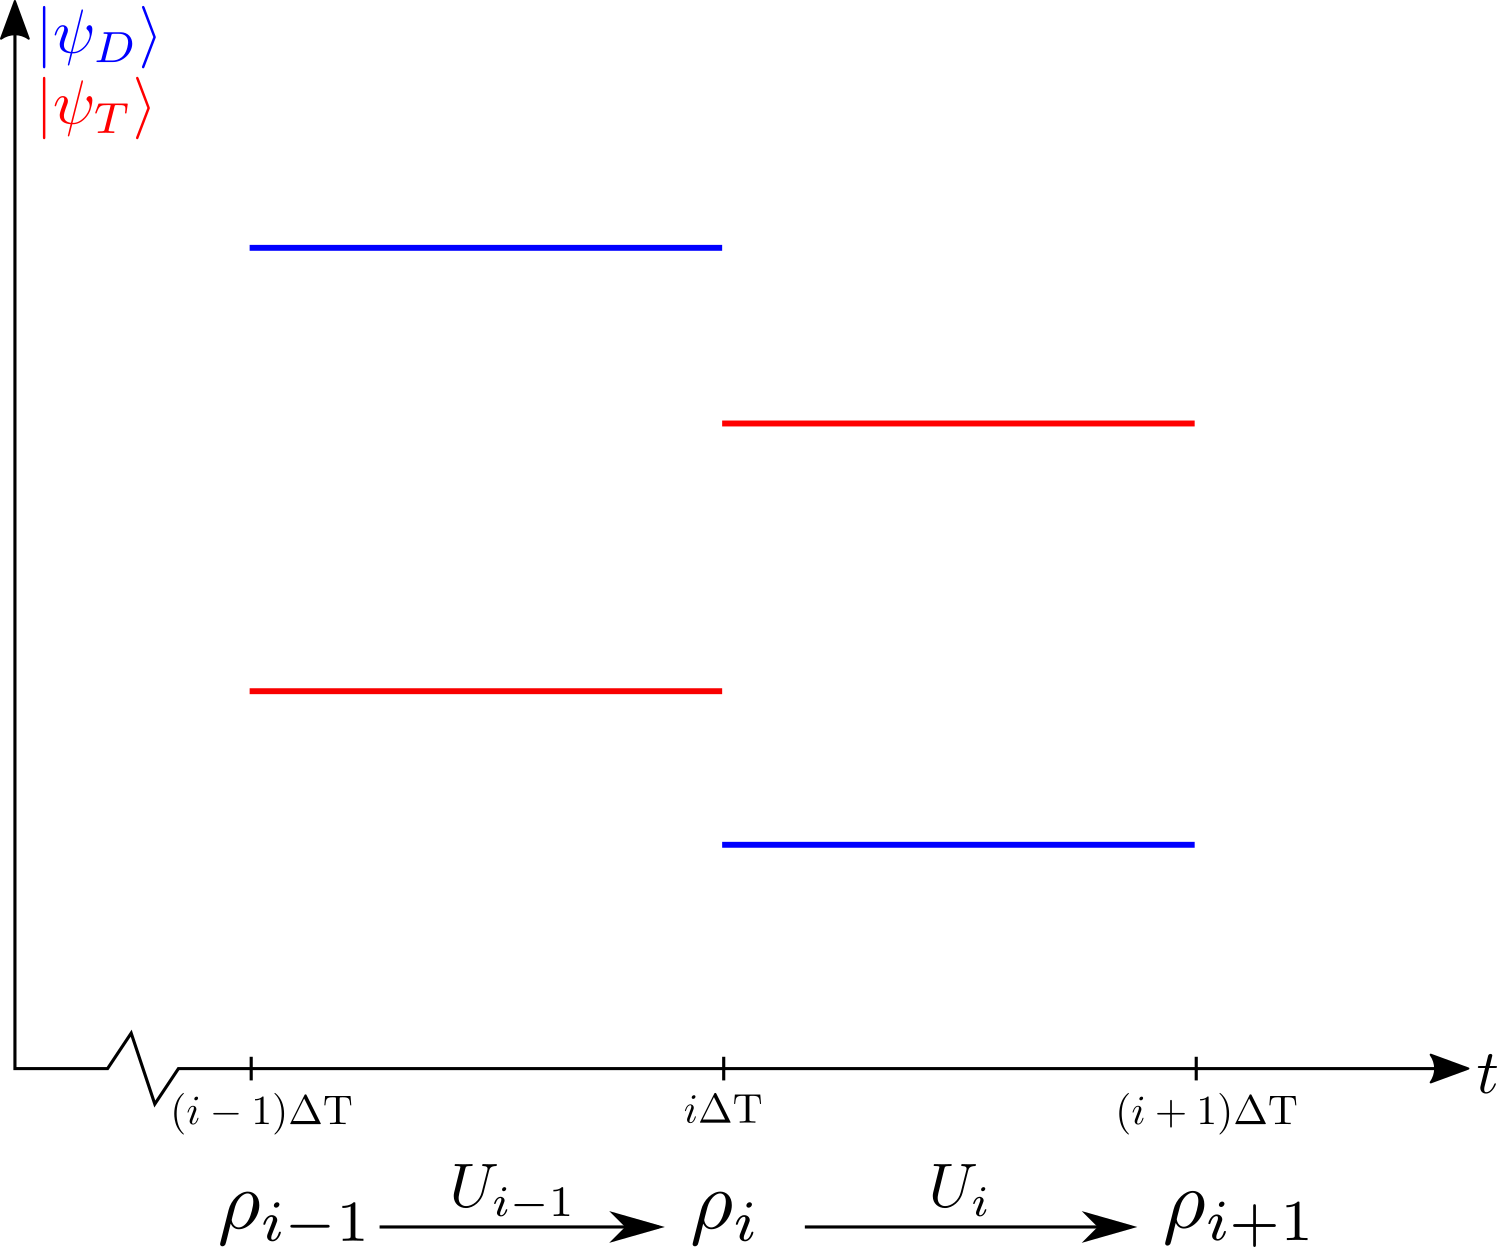
\includegraphics[width=0.6\textwidth]{img/pwc}
	\caption{Piecewise constant implementation of Drive and Transducer qubits: the vertical axis shows qubit state in arbitrary units. The qubit states are switched instantaneously and then kept constant for $\Delta \mathrm{T}$ while $\rho_S$ evolves unitarily.}
	\label{pwc}
\end{figure}

\begin{figure}
	\centering
	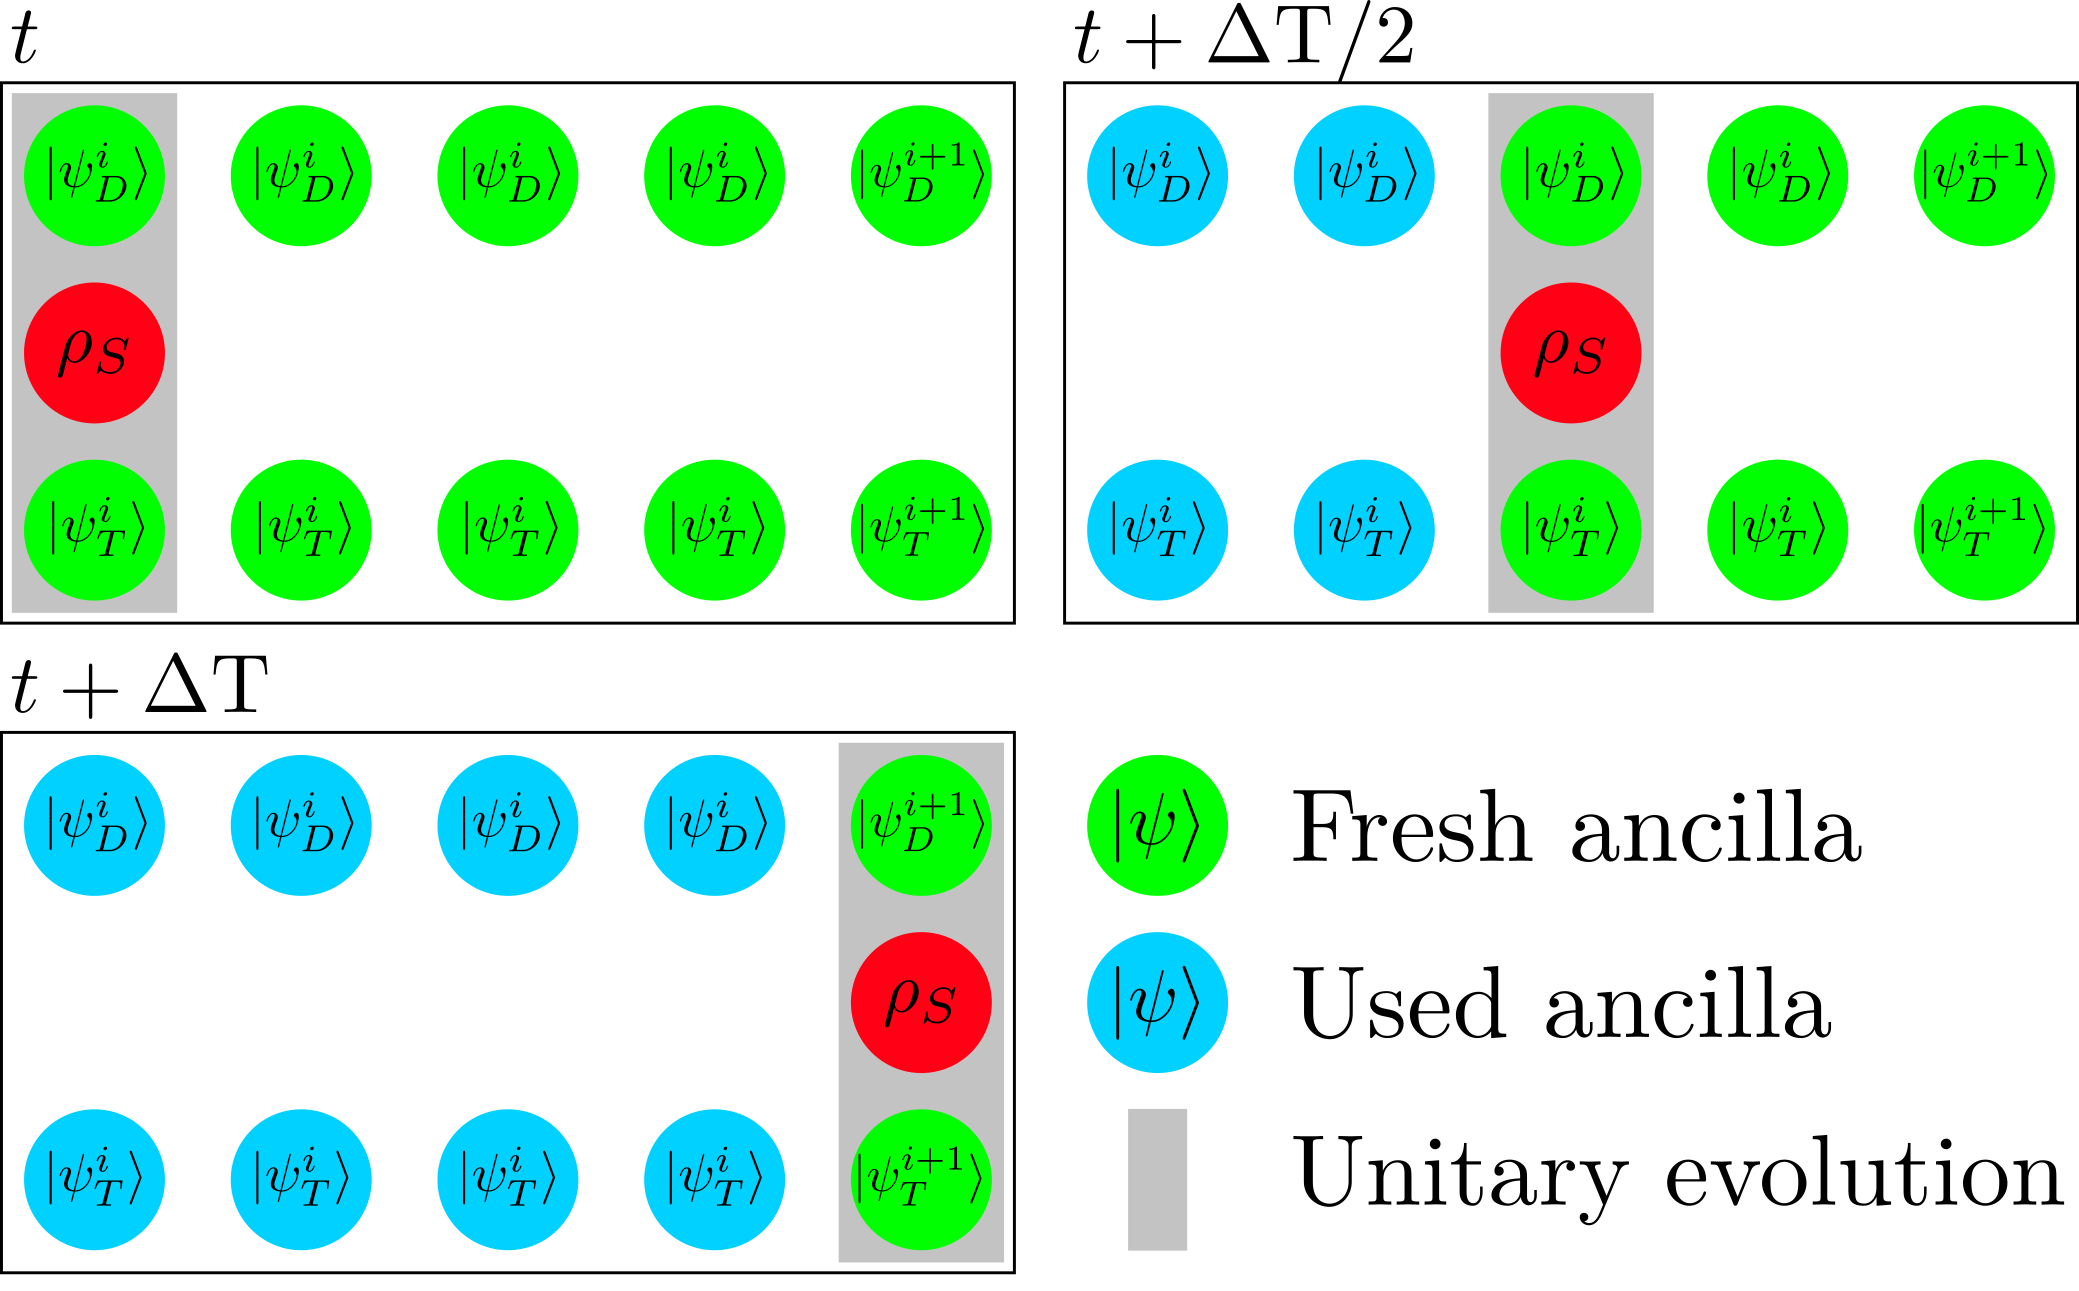
\includegraphics[width=0.7\textwidth]{img/collision_model}
	\caption{Collision model used in this work: Drive and Transducer are series of qubits interact once with the system and evolve the reduced density operator $\rho_S$. The qubit configuration can be changed in intervals of $\Delta \mathrm{T}$.}
	\label{collmodel}
\end{figure}

\cite{bernardo2020unravelling}

\chapter{Experimental Results}

\chapter{Summary and Outlook}


\bibliography{biblio}

% Erklärung
\clearpage
\thispagestyle{empty}
\minisec{Erklärung}\vspace*{1.5em}

Hiermit erkläre ich, dass ich diese Arbeit im Rahmen der Betreuung am Institut
für Theoretische Physik ohne unzulässige Hilfe Dritter verfasst und alle Quellen als solche gekennzeichnet habe.

\vspace*{45em}

Felix Soest \par
Dresden, Monat 2019

\end{document}
